\documentclass[a4paper,11pt]{article}

\usepackage[english]{babel} 
\usepackage[utf8]{inputenc}
\usepackage[cyr]{aeguill}
\usepackage{stmaryrd}

\usepackage{lmodern} %Type1-font for non-english texts and characters
\usepackage{caption}
\usepackage{subcaption}

\usepackage{graphicx}
\usepackage{hyperref}
\usepackage{listings}

\usepackage{epstopdf}

%% Math Packages 
\usepackage{amsmath}
\usepackage{amsthm}
\usepackage{amsfonts}
\usepackage{amssymb}
\usepackage{mathrsfs}
\usepackage{pst-all}
\usepackage{lscape}
\usepackage{pdfpages}
\usepackage{mathabx}


\usepackage{color, colortbl}
\definecolor{lightgray}{gray}{0.85}
\usepackage{multirow}
\usepackage[Algorithme]{algorithm}
\usepackage[noend]{algpseudocode}
\usepackage{tikz}

%\renewcommand{\algorithmicdo}{\textbf{faire}}
%\renewcommand{\algorithmicwhile}{\textbf{tant que}}


\usepackage{a4wide} %%Smaller margins = more text per page.
\usepackage{fancyhdr} %%Fancy headings

\setcounter{secnumdepth}{5}
\setcounter{tocdepth}{5}


\DeclareMathOperator*{\argmax}{arg\,max}
\DeclareMathOperator*{\argmin}{arg\,min}
\graphicspath{{/Users/melisandezonta/Documents/Documents/Documents/GTL_courses_second_semester/Computer-Vision/PS4-all/PS4-input/}}




\usepackage{listings}
\usepackage{color}
 
\definecolor{codegreen}{rgb}{0,0.6,0}
\definecolor{codegray}{rgb}{0.5,0.5,0.5}
\definecolor{codepurple}{rgb}{0.58,0,0.82}
\definecolor{backcolour}{rgb}{0.95,0.95,0.92}
 
\lstdefinestyle{mystyle}{
    backgroundcolor=\color{backcolour},   
    commentstyle=\color{codegreen},
    keywordstyle=\color{magenta},
    numberstyle=\tiny\color{codegray},
    stringstyle=\color{codepurple},
    basicstyle=\footnotesize,
    breakatwhitespace=false,         
    breaklines=true,                 
    captionpos=b,                    
    keepspaces=true,                 
    numbers=left,                    
    numbersep=5pt,                  
    showspaces=false,                
    showstringspaces=false,
    showtabs=false,                  
    tabsize=2
}
 
\lstset{style=mystyle}

\begin{document}

%\pagestyle{fancy}

\begin{titlepage}
\vspace*{\stretch{1}}

\begin{center}

\includegraphics[scale=0.4]{GT_logo.jpeg}
\end{center}
\vspace*{\stretch{1}}
\hrulefill
\begin{center}\bfseries\huge
   Computer Vision \\
   CS 6476 , Spring 2018\\
   \end{center}
  \begin{center}\bfseries\large
     PS 4\\
    \hrulefill
\end{center}
%\hfill
\vspace*{1cm}
\begin{minipage}[t]{0.6\textwidth}
  \begin{flushleft} \large
    \emph{Professor : }\\
    Cedric Pradalier \\
  \end{flushleft}
\end{minipage}
\begin{minipage}[t]{0.3\textwidth}
  \begin{flushright} \large
    \emph{Author :} \\
    Melisande Zonta \\
  \end{flushright}
\end{minipage}
\vspace*{\stretch{2}}
\begin{flushright}
       \today 
\end{flushright} 
\end{titlepage}

\tableofcontents
\clearpage




\section{Harris Corners}

\subsection{Intensity Gradients Computation}


The X/Y gradients for the two pairs of images (simA/simB and transA/transB) are respectively presented in Figure 1a and Figure 1b.

 \begin{figure}[H]
\begin{center}
\begin{tabular}{c}
	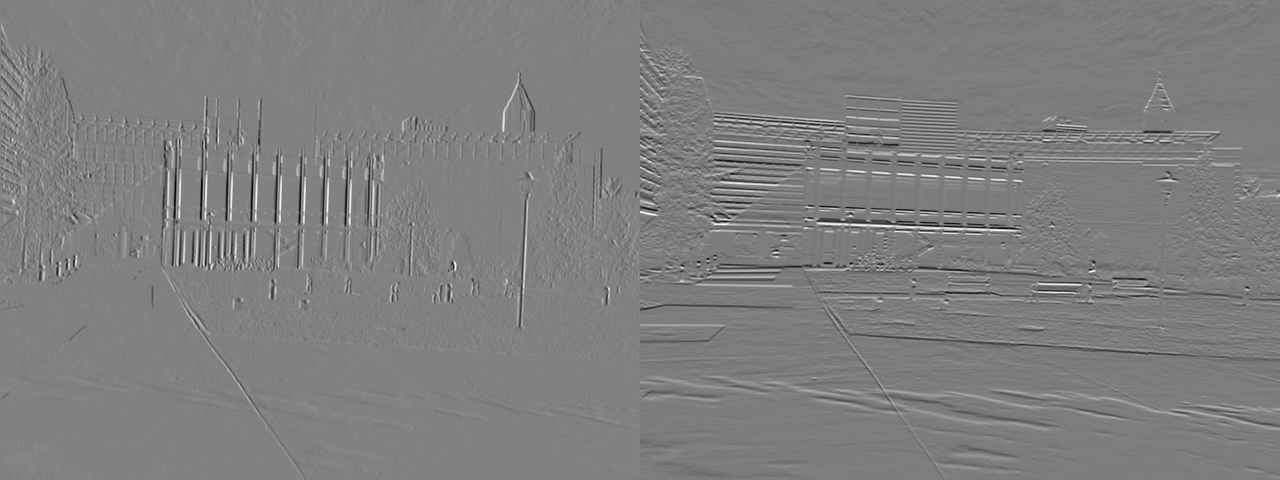
\includegraphics[width=1\textwidth]{ps4-1-1-simA.png}\\
	a\\
	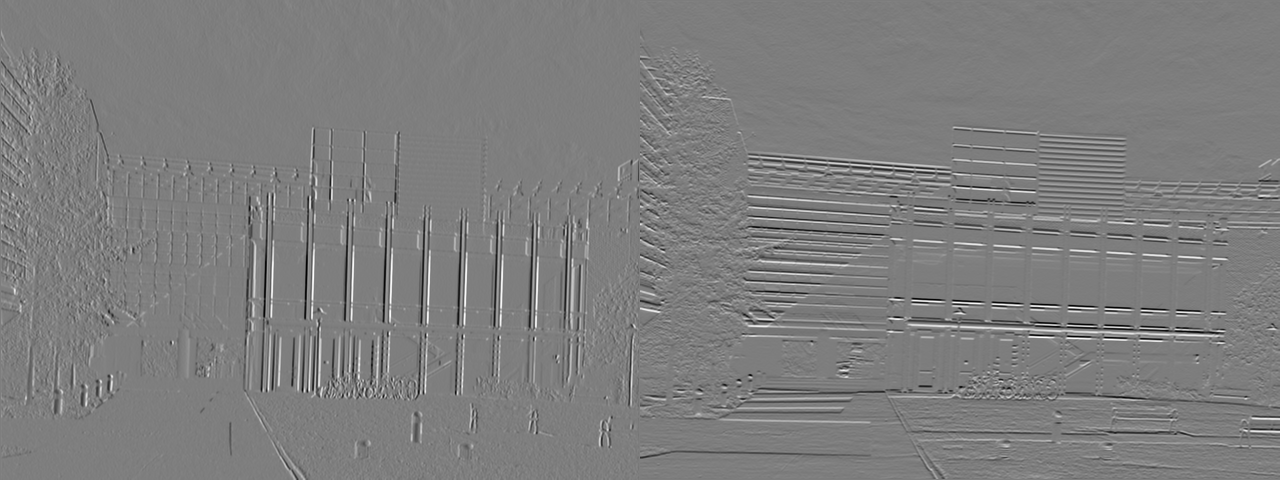
\includegraphics[width=1\textwidth]{ps4-1-1-transA.png}\\
	b
\end{tabular}
\end{center}
\caption{ 
\textit{a}. ps4-1-1-simA.  \textit{b}. ps4-1-1-transA. }
\label{ps-2-3}
\end{figure}

\lstset{style=mystyle}
\lstinputlisting[language=Python, firstline=7, lastline=17]{/Users/melisandezonta/Documents/Documents/Documents/GTL_courses_second_semester/Computer-Vision/PS4-all/PS4-code/Functions.py}

\subsection{Harris Value Computation}


The Figures 2.a,b,c,d present respectively the Harris value for simA, simB, transA and transB.
The weights used for the computation correspond to a Gaussian kernel of size 5 (thus accounting for the 24 surrounding pixels in the sum). The Harris scoring is done using ? = 0.04 which is the default value used in the OpenCV implementation (cornerHarris).

The formula we applied in the following code is :
 \begin{figure}[H]
\begin{center}
	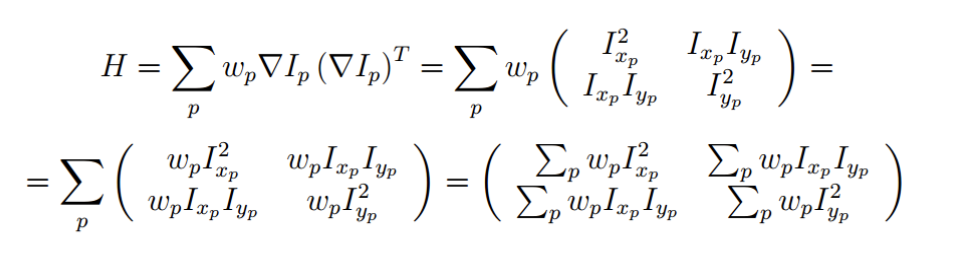
\includegraphics[width=.5\textwidth]{/Users/melisandezonta/Documents/Documents/Documents/GTL_courses_second_semester/Computer-Vision/PS4-all/Harris_corner}
\end{center}
\end{figure}

 \begin{figure}[H]
\begin{center}
\begin{tabular}{cc}
	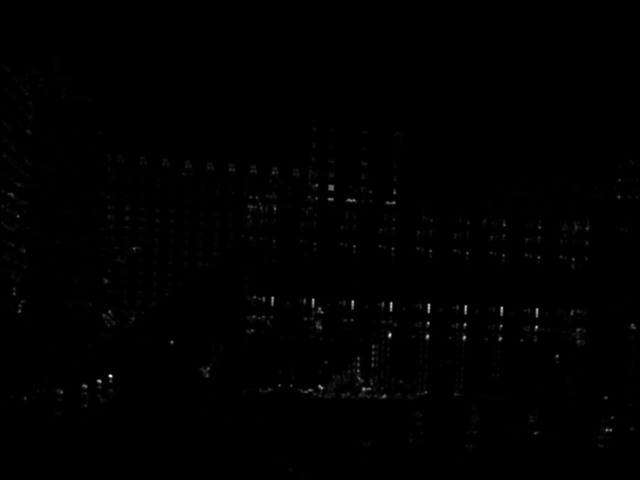
\includegraphics[width=.5\textwidth]{ps4-1-2-transA.png}&
	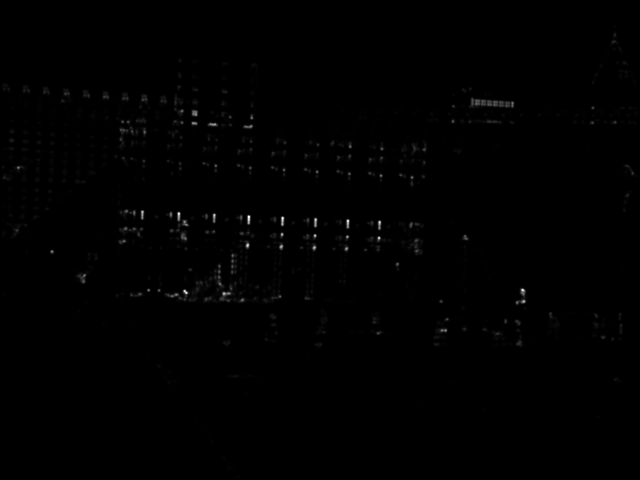
\includegraphics[width=.5\textwidth]{ps4-1-2-transB.png}\\
	a&b\\
	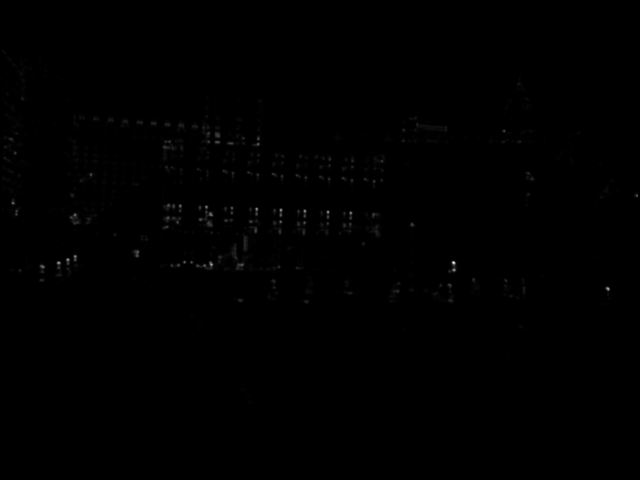
\includegraphics[width=.5\textwidth]{ps4-1-2-simA.png}&
	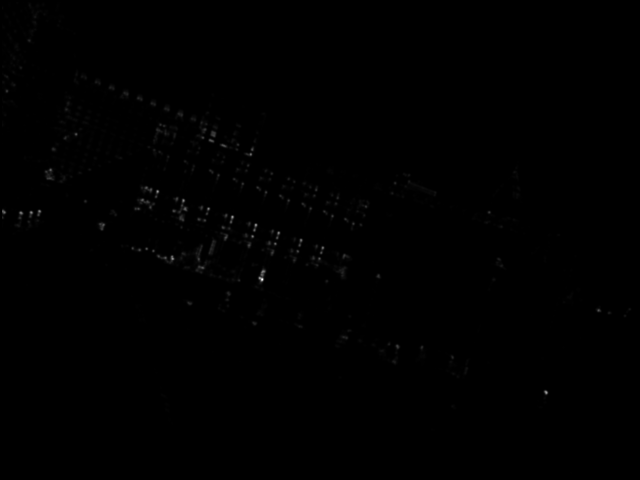
\includegraphics[width=.5\textwidth]{ps4-1-2-simB.png}\\
	c&d
\end{tabular}
\end{center}
\caption{ 
\textit{a}. ps4-1-2-transA.  \textit{b}. ps4-1-2-transB. \textit{c}. ps4-1-2-simA.  \textit{d}. ps4-1-2-simB.  }
\label{ps-4-1-2}
\end{figure}


\lstset{style=mystyle}
\lstinputlisting[language=Python, firstline=21, lastline=58]{/Users/melisandezonta/Documents/Documents/Documents/GTL_courses_second_semester/Computer-Vision/PS4-all/PS4-code/Functions.py}


\subsection{Harris Value Filtering}

The filtering of the Harris value is achieved using a combination of thresholding and non-maximum suppression.\\
To begin with, every point of the matrix below the threshold is put to zero. Then, the current maximum is found and recorded as a detected corner while its value in the matrix is set to 0, along with all the points lying in the window around (non-maximum suppression).
The resulting list of coordinates is used to draw circles around each detected corner on the original image, as shown in Figures 3.a, b, c and d.\\

 \begin{figure}[H]
\begin{center}
\begin{tabular}{cc}
	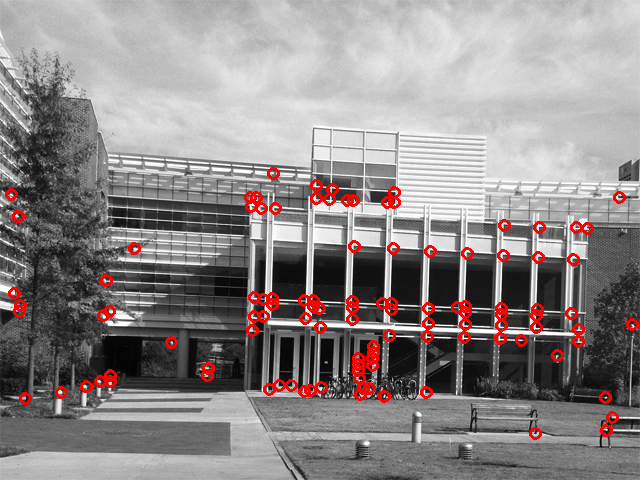
\includegraphics[width=.5\textwidth]{ps4-1-3-transA.png}&
	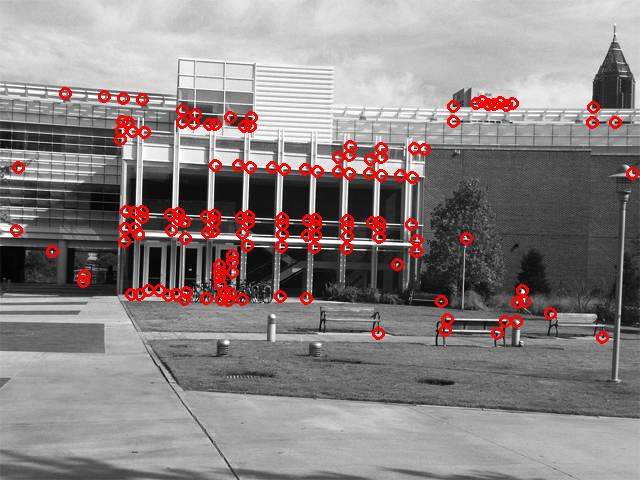
\includegraphics[width=.5\textwidth]{ps4-1-3-transB.png}\\
	a&b\\
	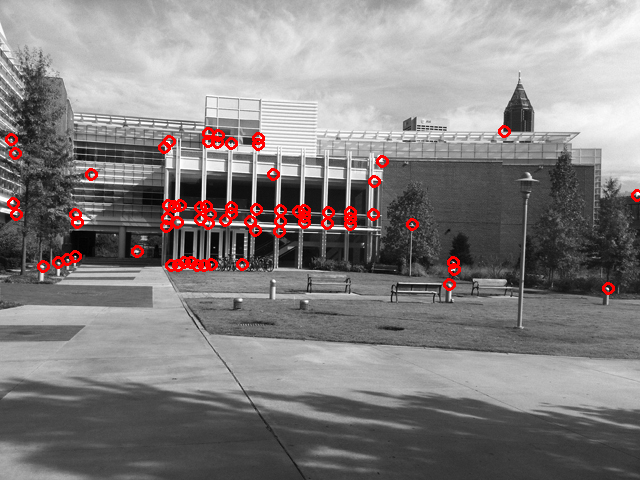
\includegraphics[width=.5\textwidth]{ps4-1-3-simA.png}&
	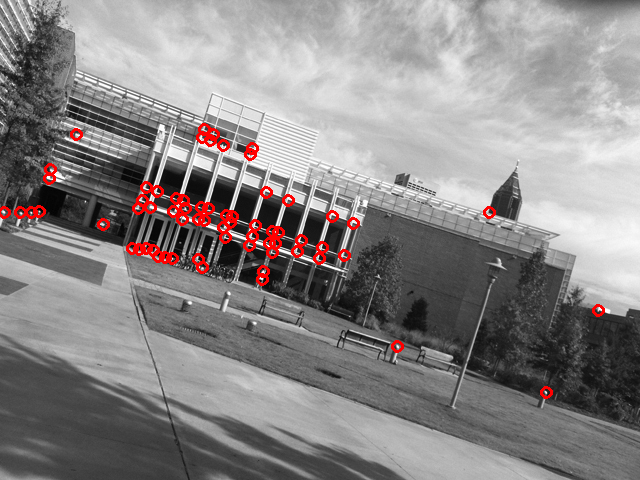
\includegraphics[width=.5\textwidth]{ps4-1-3-simB.png}\\
	c&d
\end{tabular}
\end{center}
\caption{ 
\textit{a}. ps4-1-3-transA.  \textit{b}. ps4-1-3-transB. \textit{c}. ps4-1-3-simA.  \textit{d}. ps4-1-3-simB.  }
\label{ps-4-1-3}
\end{figure}

We notice that some pixels belonging to the same physical object do not appear exactly the same on the two images of a pair.
This is particularly true for the translational case, where the number of detected corners (using the same Harris and filtering parameters) differs quite a lot. This difference cannot be simply explained by the extra corners detected on the right image that were invisible on the left one. We see for example many new matches on the building's facade, where some of the corners at the pylons get detected twice on the right, while new corners appear at the top and among the bicycles.\\
This could be explained by a slight change in lighting and shadowing which has quite a large effect on the detection which appears to be very sensitive to those.\\
Dual detection of corners does not seem worrying since we skipped corners too close to each other using the non-maximum suppression window. This will be accounted for in the RANSAC, supposing we use a threshold during this step that is equal or smaller to the non-maximum suppression window during the consensus voting.\\
The detection of corners for the similarity case leads to approximately the same number of corners detected. We can see some differences though, with a few new detection on the building?s facade and in the grass. One noticeable one is the background street lamp that is no longer detected on the second image. The intensity of the top part is noticably lower, probably due to a lighting variation.


\lstset{style=mystyle}
\lstinputlisting[language=Python, firstline=61, lastline=93]{/Users/melisandezonta/Documents/Documents/Documents/GTL_courses_second_semester/Computer-Vision/PS4-all/PS4-code/Functions.py}


\section{SIFT features}

\subsection{Gradient Orientation Computation}


The direction of the gradients is simply computed by taking the two gradient intensity matrices computed at the previous step.
The gradient orientation is then represented on the image using simple arrows.
Figure 4a, b show the result for the similarity pair while Figure 4c, d are for the translation pair.

 \begin{figure}[H]
\begin{center}
\begin{tabular}{cc}
	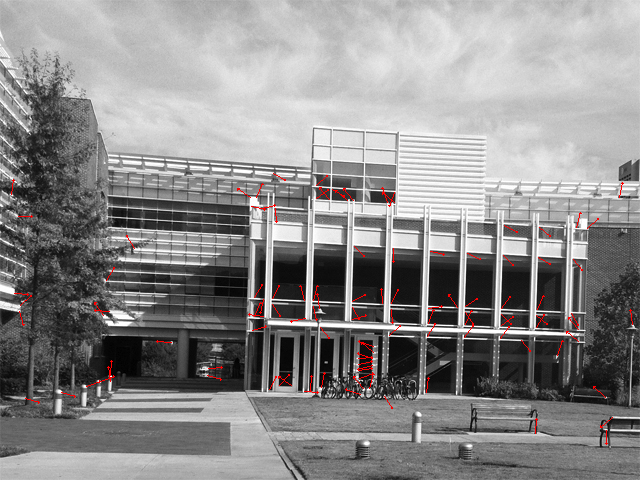
\includegraphics[width=.5\textwidth]{ps4-2-1-transA.png}&
	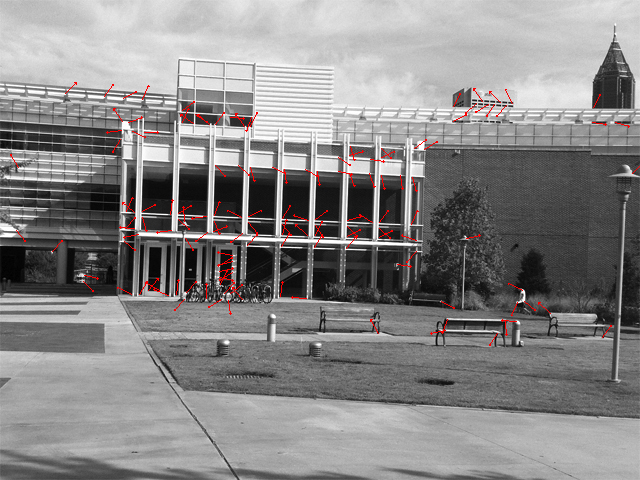
\includegraphics[width=.5\textwidth]{ps4-2-1-transB.png}\\
	a&b\\
	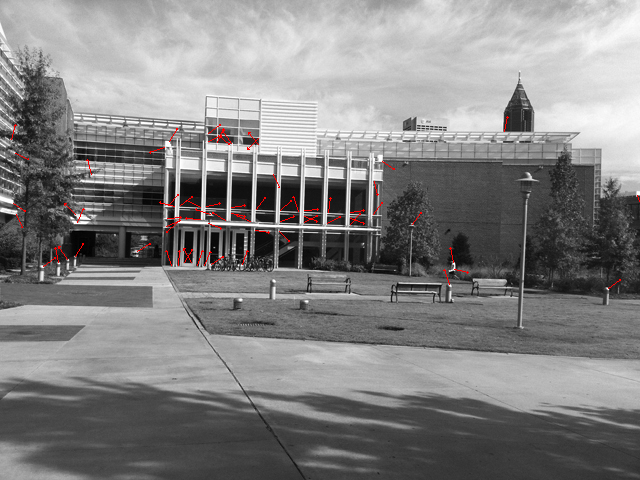
\includegraphics[width=.5\textwidth]{ps4-2-1-simA.png}&
	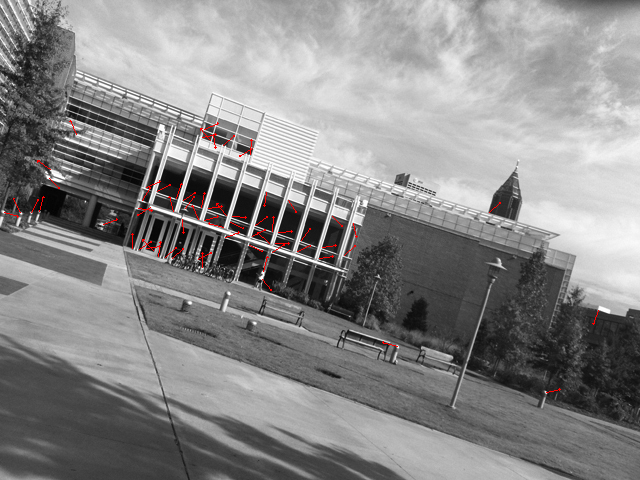
\includegraphics[width=.5\textwidth]{ps4-2-1-simB.png}\\
	c&d
\end{tabular}
\end{center}
\caption{ 
\textit{a}. ps4-2-1-transA.  \textit{b}. ps4-2-1-transB. \textit{c}. ps4-2-1-simA.  \textit{d}. ps4-2-1-simB.  }
\label{ps-4-2-1}
\end{figure}

\lstset{style=mystyle}
\lstinputlisting[language=Python, firstline=102, lastline=112]{/Users/melisandezonta/Documents/Documents/Documents/GTL_courses_second_semester/Computer-Vision/PS4-all/PS4-code/Functions.py}


\subsection{SIFT}

The matching process using SIFT is done following several steps:
\begin{enumerate}
\item Keypoints objects are created based on the corners data (positions and orientations) ;
\item Descriptors are extracted using the SIFT compute method available in OpenCV ;
\item The descriptors are matched using the brute-force matcher available in OpenCV ;
\item A putative-pair image is generated, drawing lines in different colors (generated from the HSV space) to link matched descriptors in the two images.
\end{enumerate}
The resulting putative-pair image for the similarity case is visible in Figure 5.a while Figure 5.b corresponds to the translational case.

 \begin{figure}[H]
\begin{center}
\begin{tabular}{cc}
	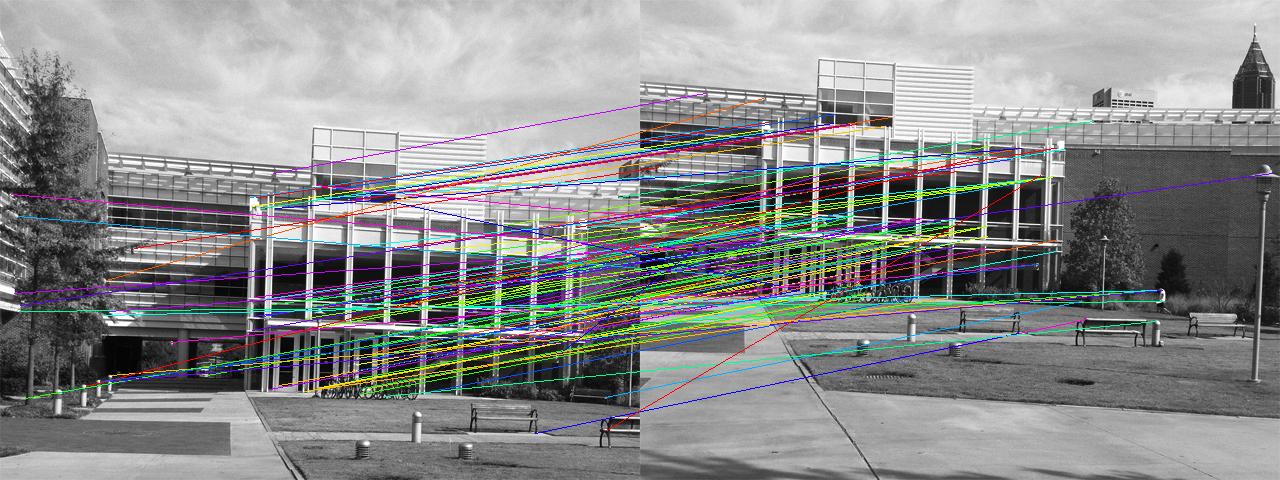
\includegraphics[width=1\textwidth]{ps4-2-2-transA-transB.png}\\
	a
	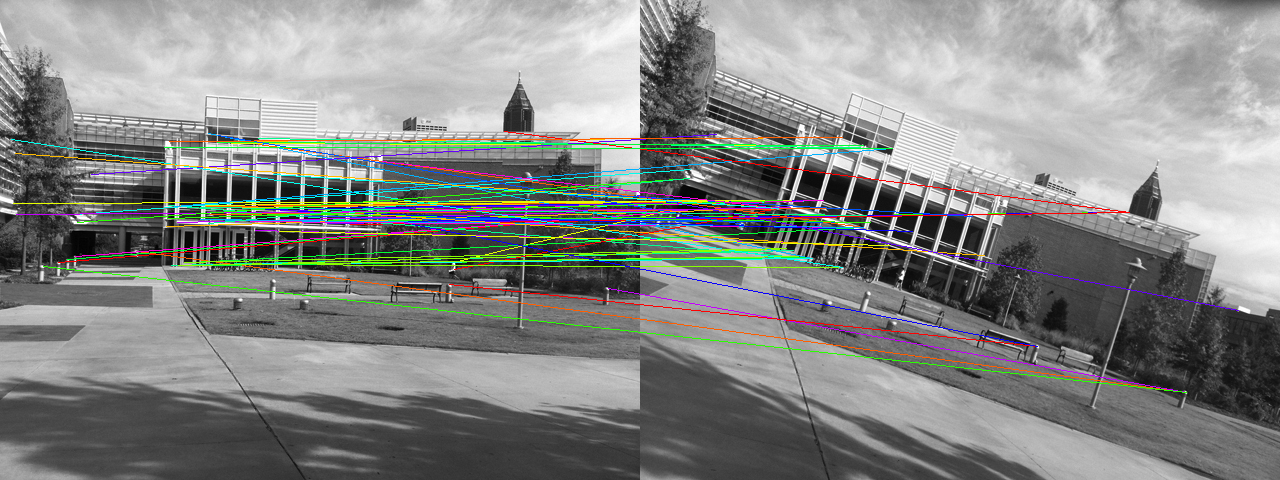
\includegraphics[width=1\textwidth]{ps4-2-2-simA-simB.png}\\
	b
\end{tabular}
\end{center}
\caption{ 
\textit{a}. ps4-2-2-transA-transB.  \textit{b}. ps4-2-2-simA-simB.  }
\label{ps-4-2-2}
\end{figure}


\lstset{style=mystyle}
\lstinputlisting[language=Python, firstline=116, lastline=165]{/Users/melisandezonta/Documents/Documents/Documents/GTL_courses_second_semester/Computer-Vision/PS4-all/PS4-code/Functions.py}


\section{RANSAC}

\subsection{RANSAC for Translation}

The translational case for RANSAC consists in randomly taking a pair of matching keypoints, computing the (dx, dy) translation parameters and checking how many other pairs match this translation parameters (for a given tolerance value).\\
Using a tolerance of 10 pixels in the consensus computation we get the following result (represented in Figure 6.a):
The best translation is $dx = 139$ and $dy = 95$ with 23 matches ($21.1\%$)
In order to get a better idea of how well the transformation applies, we use a custom function to draw the images on top of each other, which results in Figure 6.b.
We notice that although the junction looks pretty good on the ground portion at the left, other parts mismatch completely, as top left part of the building.
A variation in the mismatch seems strange considering the fact that the transformation between the left and right images is purely translational.
One possible explanation could be some kind of distorsion in the image, or a non-purely translational transformation.


 \begin{figure}[H]
\begin{center}
\begin{tabular}{cc}
	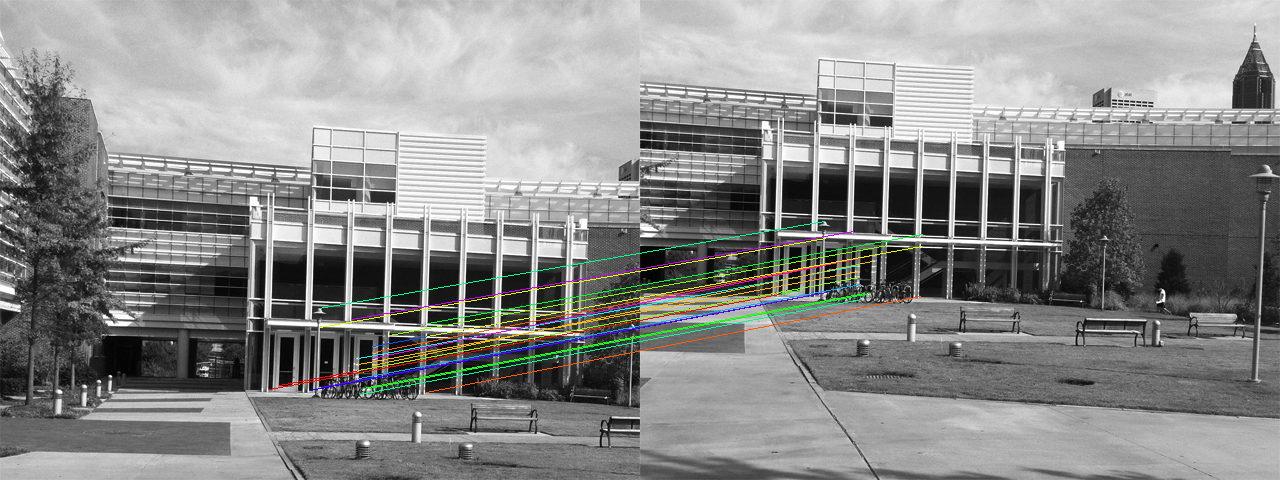
\includegraphics[width=1\textwidth]{ps4-3-1-transA-transB-a.png}\\
	a
	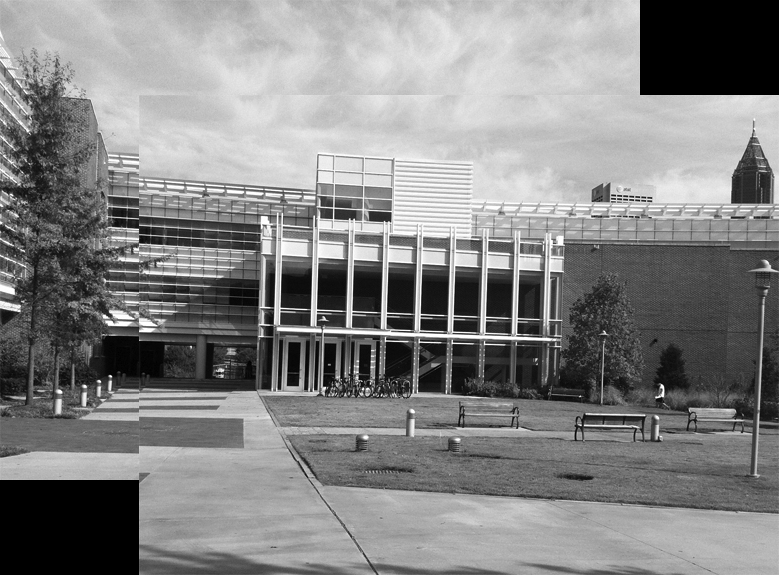
\includegraphics[width=1\textwidth]{ps4-3-1-transA-transB-b.png}\\
	b
\end{tabular}
\end{center}
\caption{ 
\textit{a}. ps4-3-1-transA-transB-lines.  \textit{b}. ps4-3-1-transA-transB-result.  }
\label{ps-4-3-1}
\end{figure}


\lstset{style=mystyle}
\lstinputlisting[language=Python, firstline=167, lastline=212]{/Users/melisandezonta/Documents/Documents/Documents/GTL_courses_second_semester/Computer-Vision/PS4-all/PS4-code/Functions.py}

\subsection{RANSAC for Similarity}

The similarity transformation case for RANSAC uses the same general method as the translational case.
However, since computing the transformation now requires a set of two pairs of matching keypoints, we take a random sample from the list of all the combinations of matched pairs.
 
We then compute the 4 parameters (a,b,c,d) of the similarity transform using a least-square method, which gives us the similarity matrix. We then compute the consensus set (for a given tolerance value) and return the matrix that corresponds to the largest set.
Using a tolerance of 3 pixels in the consensus computation we get the following result (represented in Figure 7.a):
 \begin{figure}[H]
\begin{center}
	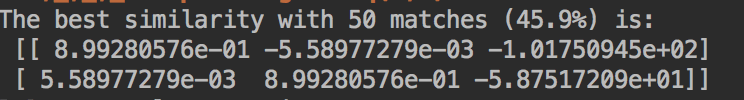
\includegraphics[width=1\textwidth]{result_similarity}
\end{center}
\end{figure}

In order to get a better idea of how well the transformation applies, we use a custom function to draw the images on top of each other, which results in Figure 7.b. The interpolation of pixels was not taken into account in this function since the idea was simply to get a rough idea of the matching.
We notice that the images here match pretty well on the left side (grass and building junctions) but give worse result on the bottom part (tree shadows and carved line in the ground). The junction in the clouds is more difficult to appreciate, because of the low contrast and the many missing pixels.
This again could be explained by a distorsion in the images, probably due to the lens of the camera.

 \begin{figure}[H]
\begin{center}
\begin{tabular}{cc}
	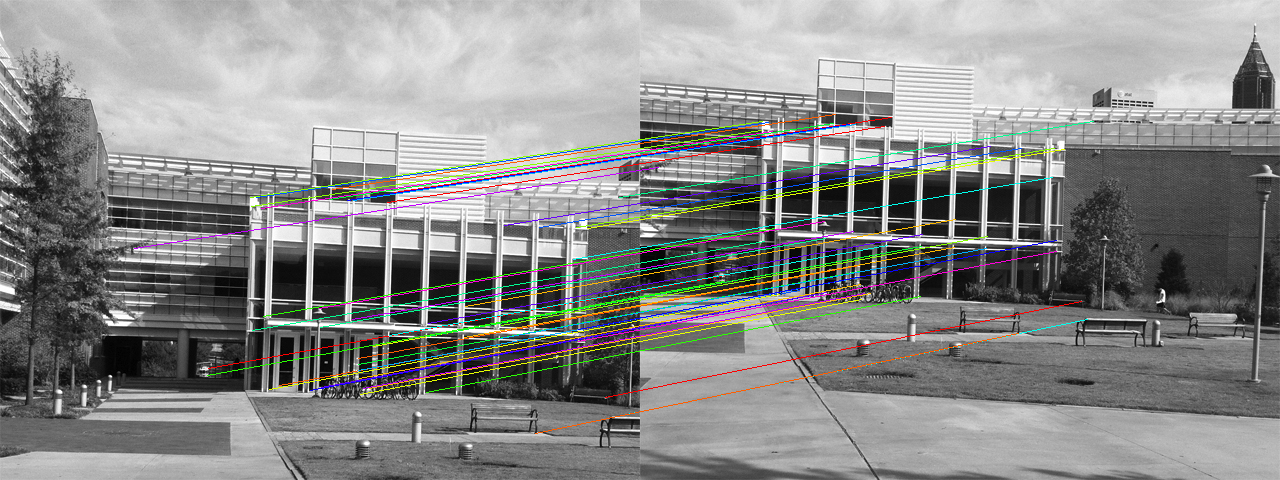
\includegraphics[width=1\textwidth]{ps4-3-2-transA-transB.png}\\
	a
	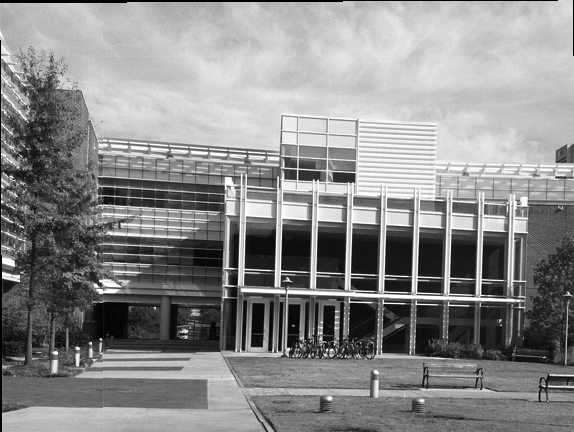
\includegraphics[width=1\textwidth]{ps4-3-2-transA-transB-result.png}\\
	b
\end{tabular}
\end{center}
\caption{ 
\textit{a}. ps4-3-2-transA-transB-lines.  \textit{b}. ps4-3-2-transA-transB-result.  }
\label{ps-4-3-2}
\end{figure}


\lstset{style=mystyle}
\lstinputlisting[language=Python, firstline=215, lastline=298]{/Users/melisandezonta/Documents/Documents/Documents/GTL_courses_second_semester/Computer-Vision/PS4-all/PS4-code/Functions.py}

\end{document}